\begin{Exercise}[title=Moment cinétique d'un satellite]
  Un satellite, assimilé à son centre d’inertie, de masse $m = 1$ tonne, décrit
  une trajectoire elliptique autour de la terre. Ce satellite n’est soumis qu’à
  la force d’interaction gravitationnelle $\vec{F}$ dirigée vers le centre de
  force$0$, centre d’inertie de la Terre. Le référentiel
  géocentrique$\mathcal{R_g}(Oxyz)$ est supposé galiléen.
  À l’instant représenté, la vitesse du satellite dans ce
  référentiel est: \gdr{v}{14650}{\km.h^{-1}}\\
  \emph{Données: Rayon de la terre: \gdr{R_T}{6400}{km}}
  \begin{center}
    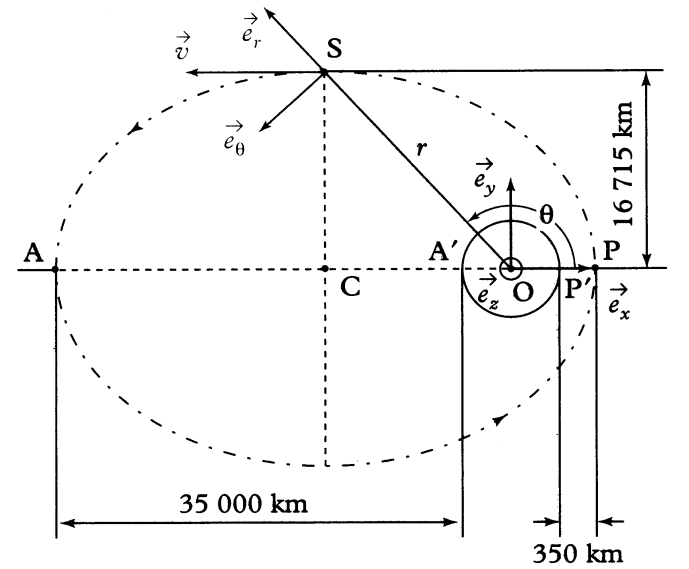
\includegraphics[width=0.4\textwidth]{satellite.png}
  \end{center}
  \Question Calculer la valeur du moment cinétique du satellite en $O$ dans
  $\mathcal{R_g}$ à l'instant considéré.
  \Question Donner la valeur de la vitesse du satellite:
  \subQuestion à son apogée A
  \subQuestion à son périgée P

\end{Exercise}
\begin{Answer}
  \Question \gdr{L_0}{6.8e13}{\kg\m^2\per\s}
  \Question
  \subQuestion $v_A=\frac{L_0}{m(AA'+R_T)}$\gdr{}{5.9e3}{\km.h^{-1}}
  \subQuestion $V_B=\frac{L_0}{m(PP'+R_T)}$\gdr{}{3.6e4}{\km.h^{-1}}
\end{Answer}
